% Viva presentation of the ANLP project 'Always Late' (course deadline 2026-10-31): one 16:9 page per slide, no beamer needed.
% Build: bash build.sh        Result slides carry \pending{...} boxes until the numbers exist; build.sh final refuses to build while any box is left.
\documentclass[10pt]{article}
\usepackage[paperwidth=13.333in,paperheight=7.5in,margin=0pt]{geometry}
\usepackage[scaled=0.95]{helvet}
\renewcommand{\familydefault}{\sfdefault}
\usepackage{courier}
\usepackage[T1]{fontenc}
\usepackage[utf8]{inputenc}
\usepackage{tikz}
\usetikzlibrary{positioning,arrows.meta,calc}
\usepackage{xcolor,booktabs,array,graphicx,enumitem}
\usepackage{fix-cm}
\pagestyle{empty}\setlength{\parindent}{0pt}
\definecolor{ink}{HTML}{14213D}\definecolor{muted}{HTML}{5C677D}\definecolor{blue}{HTML}{2A78D6}\definecolor{orange}{HTML}{EB6834}\definecolor{green}{HTML}{1BAF7A}\definecolor{pale}{HTML}{EEF3FA}
\graphicspath{{figures/}}
\newcommand{\body}[1]{\fontsize{21}{29}\selectfont #1}
\setlist[itemize]{leftmargin=1.2em,itemsep=0.45em,topsep=0.2em}
% a slide: title at the top, content in a box of 12.1 x 5.6 inches, a footer with the page number
\newenvironment{slide}[1]{\clearpage\begin{tikzpicture}[remember picture,overlay]
 \fill[pale] (current page.north west) rectangle ([yshift=-1.05in]current page.north east);
 \fill[blue] ([yshift=-1.05in]current page.north west) rectangle ([yshift=-1.10in]current page.north east);
 \node[anchor=west,text=ink,font=\fontsize{27}{30}\selectfont\bfseries] at ([xshift=0.6in,yshift=-0.55in]current page.north west) {#1};
 \node[anchor=east,text=muted,font=\small] at ([xshift=-0.5in,yshift=0.3in]current page.south east) {\thepage};
 \node[anchor=west,text=muted,font=\small] at ([xshift=0.6in,yshift=0.3in]current page.south west) {Always Late \textbullet\ ANLP 2026};
 \end{tikzpicture}\par\vspace*{1.35in}\noindent\hspace*{0.6in}\begin{minipage}[t][5.3in][t]{12.1in}\body}{\end{minipage}}
\newcommand{\pending}[1]{\par\vspace{0.4em}\fcolorbox{orange}{white}{\parbox{11.6in}{\textcolor{orange}{\textbf{RESULT PENDING}} #1}}\par}
\newcommand{\key}[1]{\textcolor{blue}{\textbf{#1}}}
\newcommand{\smallfont}{\fontsize{14}{18}\selectfont}

\begin{document}
\thispagestyle{empty}
\begin{tikzpicture}[remember picture,overlay]
 \fill[ink] (current page.north west) rectangle (current page.south east);
 \node[anchor=west,text=white,font=\fontsize{40}{46}\selectfont\bfseries,align=left] at ([xshift=0.9in,yshift=-2.6in]current page.north west) {Do interventions on language features\\survive weight quantization?};
 \node[anchor=west,text=white!80!ink,font=\fontsize{20}{26}\selectfont,align=left] at ([xshift=0.9in,yshift=-4.3in]current page.north west) {Activation survival, language association and causal effects\\in Gemma-2-2B with a Gemma Scope SAE, 27 languages};
 \node[anchor=west,text=white!70!ink,font=\fontsize{16}{20}\selectfont,align=left] at ([xshift=0.9in,yshift=-6.1in]current page.north west) {Hemang Joshi \textbullet\ Eashaan Thakur \textbullet\ Shardul Joshi \textbullet\ Nikhita Ravi\\IIIT Hyderabad \textbullet\ Advanced NLP \textbullet\ viva, October 2026};
\end{tikzpicture}

\begin{slide}{The question}
\begin{itemize}
 \item Duan et al.\ (2026) measure how much of a sparse autoencoder (SAE) feature's \key{activation} survives when the model's weights are quantized, and leave open whether interventions built on those features survive.
 \item Our setting: \key{language-selective features} of Gemma-2-2B at layer 12, 27 languages, round-to-nearest (RTN) weight quantization.
 \item A feature whose activation moves can still do the same thing, and a feature whose activation is intact can do something else.
 \item \textbf{Question:} when the weights are quantized, does the \emph{effect} of a fixed SAE-feature intervention change, and is that change due to the \emph{context} (activations before the edit), the \emph{weights} (the layers after it), or both?
\end{itemize}
\end{slide}

\begin{slide}{Setting}
\begin{itemize}
 \item Model: Gemma-2-2B; layer-12 residual; Gemma Scope SAE with 16,384 features (canonical, width 16k).
 \item Quantization: RTN per output channel of the attention and MLP weights; INT16 (rounding only), INT6, INT4; the SAE is never quantized.
 \item Text: FLORES-200, 27 languages; a BOS token that is never a statistic (the \texttt{mask} regime: a pipeline detail that changes perplexity from about 16 to 457 when missing).
 \item Edits in float32, readout in float32; every cell subtracts its own unedited baseline; a zero edit must be exactly zero.
 \item Everything frozen and hashed before any quantized outcome of this study was read; amendments are dated and kept.
\end{itemize}
\end{slide}

\begin{slide}{What the earlier studies established}
{\fontsize{18}{24}\selectfont
\begin{tabular}{@{}p{3.0in}p{9.1in}@{}}
\toprule
\key{Group necessity} & zeroing a language's 64 most selective features harms that language beyond matched controls in 27 of 27 languages (0.704 nats per token [0.684, 0.723]) \\
\key{Across precision} & the dependence is kept through INT5 (retention 1.13) and larger at INT4 (2.14) \\
\key{Where damage sits} & the language groups account for at most about 3\% of the quantization loss gap \\
\key{One feature's effect} & stays within rounding noise through INT8; median cosine with full precision 0.997 / 0.988 / 0.961 / 0.839 at INT8 / 6 / 5 / 4 (floor 0.949); the same loss for a control direction \\
\key{Survival metric} & token correlation $\geq$ 0.9 misclassifies about 31\% of the functionally intact features at INT5 \\
\key{Downstream task} & confirmatory Belebele statement not met \\
\key{Second model} & Llama-3.2-1B: pre-registered verdict ``not consistent'', exploratory \\
\bottomrule
\end{tabular}}
\vspace{0.6em}\par{\smallfont \textcolor{muted}{All exploratory unless stated; one model, one layer, one SAE, RTN weights. Sources: reports/functional\_validation/RESULTS\_SUMMARY.md.}}
\end{slide}

\begin{slide}{The gap this study closes}
\begin{itemize}
 \item The earlier effect comparisons changed \emph{everything} at once: quantized activations \emph{and} quantized layers above the edit.
 \item So they cannot say whether an intervention's effect changes because the \key{context} changed or because the \key{weights} did, nor whether the two interact.
 \item The closest published work splits the \emph{loss} change into context and weight parts (Chang et al., EMNLP 2025, §6); it does not use a fixed SAE-feature intervention, a specificity control, or a held-out prediction target.
 \item \key{This study:} cross the two factors for a fixed intervention, report the interaction, compare against matched and random directions, and test whether the transfer error can be \emph{predicted} for held-out features.
\end{itemize}
\end{slide}

\begin{slide}{Design: cross the context and the weights}
\begin{minipage}[t]{6.4in}\fontsize{19}{26}\selectfont
Fixed intervention: remove the feature's full-precision decoder contribution $v$ at its active positions at layer 12.

\vspace{0.4em}$D[p,s]$ = change of the output logits (centered) when $v$ is removed, with prefix state $p$ (activations before the edit) and suffix state $s$ (weights after it); each state FP or quantized (Q).

\vspace{0.4em}$C = D[Q,FP]-D[FP,FP]$ \hfill (context)\\
$W = D[FP,Q]-D[FP,FP]$ \hfill (weights)\\
$I = D[Q,Q]-D[Q,FP]-D[FP,Q]+D[FP,FP]$ \hfill (interaction)\\
\textcolor{blue}{$D[Q,Q]-D[FP,FP]=C+W+I$} exactly, before averaging.
\end{minipage}\hfill
\begin{minipage}[t]{5.4in}\vspace{0.3in}\centering
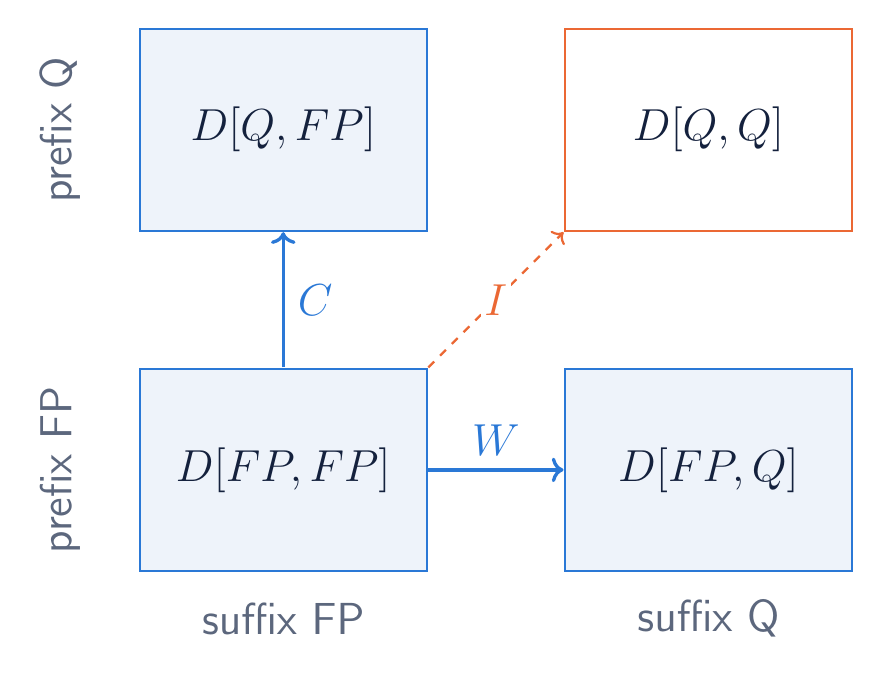
\begin{tikzpicture}[scale=1.35,transform shape,font=\fontsize{12}{15}\selectfont,cell/.style={draw=blue,fill=pale,minimum width=2.7cm,minimum height=1.9cm,text=ink,line width=0.8pt}]
 \node[cell] (ff) at (0,0) {$D[FP,FP]$}; \node[cell] (fq) at (4.0,0) {$D[FP,Q]$};
 \node[cell] (qf) at (0,3.2) {$D[Q,FP]$}; \node[cell,draw=orange,fill=white] (qq) at (4.0,3.2) {$D[Q,Q]$};
 \node[text=muted] at (0,-1.4) {suffix FP}; \node[text=muted] at (4.0,-1.4) {suffix Q};
 \node[text=muted,rotate=90] at (-2.1,0) {prefix FP}; \node[text=muted,rotate=90] at (-2.1,3.2) {prefix Q};
 \draw[->,very thick,blue] (ff.north) -- (qf.south) node[midway,right,text=blue] {$C$};
 \draw[->,very thick,blue] (ff.east) -- (fq.west) node[midway,above,text=blue] {$W$};
 \draw[->,thick,orange,dashed] (ff.north east) -- (qq.south west) node[pos=0.5,fill=white,inner sep=1pt,text=orange] {$I$};
\end{tikzpicture}\\[0.6em]{\smallfont \textcolor{muted}{Also stored: the quantized state's own activation ($D[Q,Q]$ at native amplitude).}}
\end{minipage}
\end{slide}

\begin{slide}{Directions, floor, eligibility, held-out split}
\begin{itemize}
 \item \key{Directions:} the real decoder direction; the matched swapped direction (another feature's); three random norm-matched directions orthogonal to it. Controls measure what \emph{any} direction would do.
 \item \key{Numerical floor:} even INT16 changes the logits (bfloat16 execution); the 95th percentile of the INT16 error over \emph{calibration} features, per direction kind. An item is \key{eligible} if its full-precision effect exceeds five floors (about 5\% of the items).
 \item \key{Split:} the 404 features are split by hash into calibration and held-out halves; fits, floors and the choice of the strongest baseline use calibration only; documents (the parallel source sentence) are the bootstrap clusters, features crossed.
 \item \key{Uncertainty:} 2,000 crossed bootstrap replicates, seed 20261026.
\end{itemize}
\end{slide}

\begin{slide}{Three panels}
{\fontsize{19}{25}\selectfont
\begin{tabular}{@{}p{2.6in}p{4.8in}p{4.6in}@{}}
\toprule
 & \textbf{what} & \textbf{size} \\
\midrule
\key{Feature level} & 404 language-selective features, up to 16 contexts each, 5 directions, cached residual at layer 12 & 6,464 feature--context pairs, 32,320 items per state \\
\key{Group level} & each language's K=64 group and 3 matched control groups on FLORES devtest & 27 languages $\times$ 300 sentences $\times$ 4 sets \\
\key{External panel} & Wikipedia (revision pinned), 6 languages, 64--128 token passages, fresh contexts & 1,800 passages, 402 features, 7,200 group items per state \\
\bottomrule
\end{tabular}}
\vspace{0.7em}\par{\smallfont \textcolor{muted}{States: INT16 (rounding-only reference, never a result), INT6, INT4. About 30 GPU-hours on RTX 2080 Ti nodes. The external panel is a validity check on fresh text, not a replication of the 27-language study.}}
\end{slide}

\begin{slide}{Rules fixed before the outcomes}
{\fontsize{18}{24}\selectfont
\begin{tabular}{@{}p{1.3in}p{10.6in}@{}}
\toprule
\key{A3} & the context term dominates the weight term (the interval of the median over languages of $|C|-|W|$ above zero and median $|C|>$ median $|W|$, at INT6 and INT4): the \emph{expectation} from Chang et al.; confirming it alone is not a contribution \\
\key{H1} & the error of the native effect needs more than an activation change or a rescaling: more than half the error remains after the best rescaling and after the native amplitude, and the error exceeds the numerical floor \\
\key{H2} & the crossed terms and the interaction are measured and reproducible between the calibration and the held-out half (descriptive) \\
\key{H3} & the sensitivity to \emph{other} directions predicts the transfer error beyond activation-based predictors \\
\key{H4} & the transfer of a feature's \emph{averaged} fingerprint differs from the transfer of its single contexts, by more than the rounding-only state does \\
\key{Utility} & a model with the generic sensitivity reduces the held-out error by at least 10\% against the strongest baseline, interval above zero, at INT6 and INT4 separately \\
\bottomrule
\end{tabular}}
\vspace{0.5em}\par{\smallfont \textcolor{muted}{Status words by rule: supported / reversed / inconclusive. Baselines: A activation (cosine of amplitudes, log activation, firing, effect and residual norms), G gradient attribution, B generic sensitivity from the other directions of the same context.}}
\end{slide}

\begin{slide}{Group level: for the fixed edit, the context term is larger at INT4}
{\fontsize{18}{24}\selectfont
\begin{tabular}{@{}lrrrrr@{}}
\toprule
 & net harm & $|C|$ & $|W|$ & $|I|$ & $|C|>|W|$ in\\
\midrule
INT16 (rounding) & 0.262 & 0.0005 & 0.0003 & 0.0002 & 19 of 27$^\dagger$\\
INT6 & 0.281 & 0.0091 & 0.0092 & 0.0010 & 12 of 27\\
INT4 & \textbf{0.848} & \textbf{0.310} & \textbf{0.104} & 0.071 & \textbf{19 of 27}\\
\bottomrule
\end{tabular}}
\vspace{0.6em}
\begin{itemize}
 \item Median over 27 languages, 300 sentences; net harm of removing the K64 group beyond matched controls (full precision: 0.263, as in the earlier study).
 \item INT4: net harm 0.85 with the fixed FP edit, 0.43 with the quantized state's own activation, which is the weights-only value (0.428): for the natural intervention the amplification is that of the weights. Interval of the median $|C|-|W|$: [+0.022, +0.073].
 \item \key{A3} (context dominates, for the fixed edit): supported at INT4, undecided at INT6. $^\dagger$ the count is also 19 at rounding size: the interval, not the count, is the evidence.
\end{itemize}
\end{slide}

\begin{slide}{Feature level: the effect vector is rotated; the weight term is larger}
{\fontsize{18}{24}\selectfont
\begin{tabular}{@{}lrrrrrr@{}}
\toprule
 & cosine & error & in floors & $C$ & $W$ & $I$\\
\midrule
INT16 (rounding) & 0.998 & 0.056 & 0.7 & 0.055 & 0.053 & 0.074\\
INT6 & 0.984 & 0.165 & 1.9 & 0.100 & 0.145 & 0.086\\
INT4 & \textbf{0.768} & \textbf{0.664} & \textbf{7.7} & 0.359 & \textbf{0.560} & 0.315\\
\bottomrule
\end{tabular}}
\vspace{0.4em}
\begin{itemize}
 \item 2,203 eligible items of 235 features (34\%). Terms relative to the FP effect norm plus the floor.
 \item The error is 97--99\% orthogonal to the FP effect, and the quantized state's own activation leaves 97\% of it: not a rescaling, not an activation change (\key{H1} supported).
 \item Weight term above context term in the effect vector (norm of a logit change; exploratory, the terms are not additive), the opposite of the group-level loss: different quantities. The interaction is a third of the change at INT4.
\end{itemize}
\end{slide}

\begin{slide}{Which term, is it specific, and do averages hide the contexts?}
\centering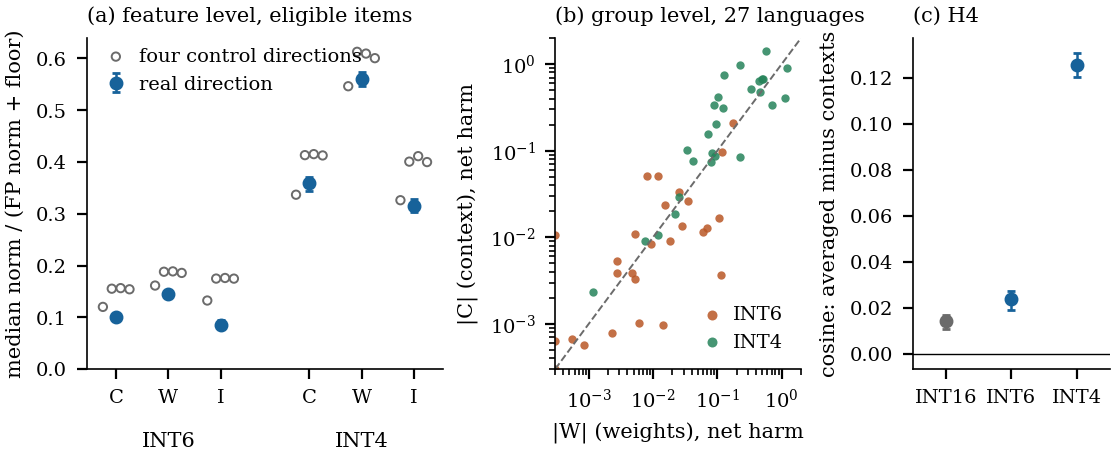
\includegraphics[width=10.0in]{transfer-terms.png}\par\vspace{0.2em}
{\fontsize{15}{19}\selectfont\raggedright\textbf{(a)} Real direction (filled) against matched and random directions (hollow): weight term above context term, and the real direction is close to its controls (INT4 error gap +0.019 [+0.009, +0.032]); at matched FP effect size (144 pairs, post hoc) its error norm is $\times$1.12 (INT6) and $\times$1.14 (INT4) that of a swapped direction, $\times$1.00 at INT16: mostly a generic response with a modest specific part. \textbf{(b)} Group level: context above weights at INT4 (green), equal at INT6. \textbf{(c)} The averaged fingerprint looks better than its contexts: +0.126 [0.121, 0.131] at INT4 against +0.0145 in the rounding-only state (\key{H4}, features-only interval).\par}
\end{slide}

\begin{slide}{Can the transfer error be predicted for held-out features?}
\begin{minipage}[t]{6.2in}\vspace{0pt}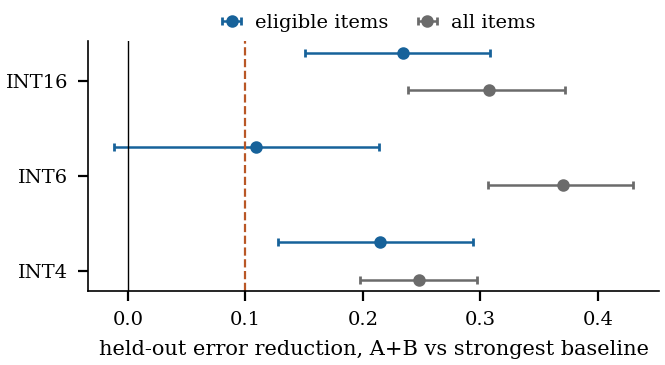
\includegraphics[width=6.1in]{transfer-predict.png}\end{minipage}\hfill
\begin{minipage}[t]{5.6in}\vspace{0pt}\fontsize{19}{26}\selectfont
A+B = activation baseline plus the sensitivity to \emph{other} directions of the same context, against the strongest baseline:\\[0.3em]
INT4: \textbf{21.5\%} [12.7, 29.4], criterion met\\
INT6: 10.9\% [$-$1.2, 21.4], interval includes zero, not met (all items: 37.1\% [30.7, 43.0])\\
INT16 (rounding only): 23.4\% [15.1, 30.8]: the gain is not quantization-specific\\[0.4em]
\key{Utility not met} (needs both states).
\end{minipage}
\end{slide}

\begin{slide}{What does not add to the prediction, and what it means}
\begin{itemize}
 \item \key{Gradient attribution} (loss form, eligible items, INT4): held-out error 0.1241 against 0.1253 without it (no interval).
 \item \key{Pearson survival} of the feature: A+P against A $-0.4\%$ [$-1.8$, 0.7] at INT4; A+B+P against A+B $-0.6\%$ [$-4.3$, 3.4]; at INT6 A+B+P is worse than A+B ($-6.5\%$ [$-12.0$, $-1.6$]).
 \item The sensitivity to other directions measures how \emph{noise-prone a context} is (it works in a rounding-only state too), not a quantization-specific mechanism.
 \item So: INT6 changes the effect little (about two numerical floors, above the rounding floor); INT4 does not (cosine 0.77); most of the transfer error is shared with other directions and hidden by averaging; activation survival is not a reliable proxy for it.
\end{itemize}
\end{slide}

\begin{slide}{Status of every pre-declared claim (rules fixed before the outcomes)}
{\fontsize{18}{24}\selectfont
\begin{tabular}{@{}p{1.6in}p{3.0in}p{6.7in}@{}}
\toprule
\key{A3} & mixed & supported at INT4, undecided at INT6 (interval spans zero)\\
\key{H1} & supported & both states; the error clears the numerical floor (1.9 and 7.7 floors)\\
\key{H2} & descriptive & calibration and held-out intervals of $C$, $W$, $I$ overlap\\
\key{H3} & mixed & supported at INT4, inconclusive at INT6\\
\key{H4} & supported & features-only interval; separates from the rounding-only state\\
\key{Utility} & not met & INT4 met, INT6 not met (interval includes zero)\\
\bottomrule
\end{tabular}}
\vspace{0.5em}\par{\fontsize{14}{18}\selectfont\textcolor{muted}{Rules tightened once after an independent code review, before any outcome was read (amendment A14). Held-out = held-out features (no document holdout). Wikipedia panel, same rules: A3 mixed, H1 supported, H3 supported, H4 mixed, utility met.}}
\end{slide}

\begin{slide}{External panel: fresh text, six languages (Wikipedia)}
{\fontsize{17}{22}\selectfont
\begin{tabular}{@{}p{2.2in}p{4.6in}p{5.4in}@{}}
\toprule
 & FLORES, 27 languages & Wikipedia, 6 languages\\
\midrule
\key{A3} context larger & INT4 supported, INT6 undecided & INT4 supported ($+0.053$ [0.040, 0.064]), \textbf{INT6 reversed} (weights larger, $-0.0049$)\\
\key{H1} not a rescaling & supported (1.9 and 7.7 floors) & supported (1.8 and 7.1 floors)\\
\key{H3} prediction & INT4 yes, INT6 no (10.9\% [$-$1.2, 21.4]) & both yes: 19.4\% [5.1, 31.8], 23.4\% [12.8, 32.5]\\
\key{H4} averages hide & supported & INT4 supported ($+0.132$), INT6 inconclusive\\
\key{Utility} (both states) & not met & \textbf{met}\\
\bottomrule
\end{tabular}}
\vspace{0.5em}
\begin{itemize}
 \item \key{Cross-corpus, no refit:} models fitted on the FLORES calibration features score the Wikipedia held-out items: 20.6\% [9.3, 31.2] at INT4, 19.7\% [7.5, 29.5] at INT6, 26.7\% in the rounding-only state.
 \item The rounding-only state is predicted as well (28.9\%): the predictor measures how noise-prone a context is, not a quantization-specific mechanism. Eligible items: 22.5\% against 34.1\%.
 \item Six languages, group medians dominated by one heavy-tailed language: an external-validity check, not a replication.
\end{itemize}
\end{slide}

\begin{slide}{What this does not show}
\begin{itemize}
 \item One model, one layer, one SAE, one quantizer (simulated RTN, not deployed integer kernels); Gemma-2-9B is run by another team and is not part of this work.
 \item The earlier descriptive studies are exploratory; the only confirmatory family (Belebele) was not met.
 \item About a third of the real-direction items (2,203 of 6,464; 235 of 404 features) clear the numerical floor; the held-out half is 1,066 items of 116 features, and the all-items tables are reported next to the eligible ones.
 \item The gradient baseline is the loss-attribution form, not the effect-vector form; Pearson survival is a secondary question.
 \item Nothing here is a statement about task accuracy, safety or deployment.
\end{itemize}
\end{slide}

\begin{slide}{Reproducibility and where to look}
\begin{itemize}
 \item Code, tests, ledger and decisions: \texttt{github.com/TH4KUR/always-late} (the zip holds the committed state).
 \item Freeze and amendments: \texttt{reports/intervention\_transfer/} (\texttt{freeze.json}, \texttt{amendment\_A*.json}, \texttt{STATUS.md}); claim rules in the docstring of \texttt{phase1\_transfer\_report.py}.
 \item Every module has tests written first and a mutation check (\texttt{scripts/g0/mutcheck.py}); every GPU job is validated against its log, gates and sha256 (\texttt{phase1\_transfer\_validate.py}).
 \item Large artifacts: private Hugging Face dataset \texttt{karma-skz/always-late-artifacts}; metrics: wandb project \texttt{karma-skz-/anlp-project}.
\end{itemize}
\end{slide}
\end{document}
